\documentclass{article}
\usepackage{pythonhighlight}
\usepackage{graphicx}
\usepackage{ctex}
\usepackage[left=3cm,top=3cm,right=3cm]{geometry}
\usepackage{hyperref}
% TITLE PAGE CONTENT %%%%%%%%%%%%%%%%%%%%%%%%
%%%%%%%%%%%%%%%%%%%%%%%%%%%%%%%%%%%%%%%%%%%%%
\newcommand{\labno}{07}
\newcommand{\labtitle}{EE208 Intergration}
\newcommand{\authorname}{周李韬}
\newcommand{\studentno}{518030910407}
\newcommand{\classno}{F1803016}
% END TITLE PAGE CONTENT %%%%%%%%%%%%%%%%%%%%


\begin{document}

\begin{center}
{\LARGE \textsc{Laboratory No. \labno:} \\ \vspace{4pt}}
{\Large \textsc{\labtitle} \\ \vspace{4pt}} 
\rule[13pt]{\textwidth}{1pt} \\ \vspace{15pt}
{\large By: \authorname \\ \vspace{10pt}
No. \studentno \\ \vspace{10pt}
SJTU \classno \\ \vspace{10pt}
\today \vspace{20pt}}
\end{center}



\section{实验准备}

\subsection{实验环境}
\begin{itemize}
\item\textbf{Environment} Ubuntu 16.04 (on Virtual Machine)
\item\textbf{Language} Python 2.7.16 with packages as follows
	\begin{itemize}
	\item urllib 1.24.2
	\item beautifulsoup4 4.8.0
	\item lucene 4.9.0
	\item web.py 3.7
	\end{itemize}
	HTML/CSS (with help of Bootstrap)
\item\textbf{Tools} PyCharm 2019.2, Virtual Box
\end{itemize}

\subsection{实验目的}

本实验中,基于此前的成果,我们需要构建一个网页+图片搜索引擎。搜索引擎的内容基于爬虫爬取的网页(本实验中对网页、图片内容分别爬取了新浪门户网站的网页内容和豆瓣电影区的图片),索引的建立与搜索基于Python中的Lucene库,前端Web框架由web.py构建。网页样式由div+CSS进行规范。

\subsection{实验原理}

在前一次的web.py初步搭建实验中,我们已经实现了搜索主页、网页搜索结果展示页的搭建。在本实验中,我们首先需要为此前建立的图片结果搜索程序搭建对应的前端展示页。接下来,我们需要通过div+CSS的方法对网页样式作一定的规范和美化。

在URL组织方面,考虑到无论是对网页还是图片,结果网页除去内容以外的其余部分排版基本是一致的,因此在web.py中我们采用了同一个模板,根据传入的参数判断生成图片结果页还是网页结果页,传入相应的数据和生成对应的格式。在表单设计上,对搜索框表单我们添加了两个单选框用于区分网页、图片搜索,单选框的值会被传入结果页生成对应的网页。在搜索程序中,索引和查询程序的框架沿用了此前的实验结果,在得到查询结果后,我们通过Python字符串的形式将结果用HTML标签连接了起来,以便于在web.py中传入模板。在页面规范方面,为提升排版的效率和效果,我们采用了Bootstrap框架,通过CSS样式表,为网页中的图片框、网页结果标题、URL、摘要等元素设置了类型,达到了有序呈现网页结果的效果。具体的实验细节将在下文详述。

\section{实验步骤}

\subsection{页面组织}

与上一次实验一致,我们依然采用了两类URL,分别匹配主页和搜索结果展示页,对应两类页面模板。
\begin{python}
urls = (
    '/', 'index',
    '/s', 's',
)
\end{python}

与此前实验不同之处在于,为了便于规范格式和排布,我们直接在模板HTML文件中加入了采用Bootstrap样式的表单,而没有使用web.py自动生成的form类。对应的HTML代码如下:
\begin{python}
<form class="form-group" action="/s" method="GET">
	<div class="form-inline">
			<input class="form-control" type="text" id="keyword" name="keyword"/>
			<button class="btn btn-default" id="Search" name="Search">搜索</button>
	</div>
	<div class="form-group">
		<input type="radio" id="option" value="web" name="option"/> 新浪网页
		<input type="radio" id="option" value="images" name="option"/> 豆瓣电影
	</div>
</form>
\end{python}

当表单发出GET请求时,对应搜索结果url的GET函数会记录用户选择的搜索方式,传入的关键词,根据option的不同,执行相应的搜索程序,从result模板生成对应的网页。由于表单不再通过web.py生成,模板的参数中去掉了表单。
\begin{python}
class s:
    def GET(self):
        user_data = web.input()
        option = user_data.option     % 搜索方式
        kw = user_data.keyword        % 关键词
        vm_env.attachCurrentThread()
        if (option == 'web'):
            contents = web_func(kw)   % 调用搜索程序,获取结果
            return render.result('Web',kw, contents) % 生成网页
        else :
            contents = img_func(kw)
            return render.result('Img',kw, contents)
\end{python}

\subsection{主页的布局}

\paragraph{搜索表单} 本实验中,搜索表单通过调用了Bootstrap库中的样式实现,在HTML中,表单位于一个id为idx的容器中,我们通过CSS样式表为容器添加了半透明的背景和页面居中的属性。
\begin{python}
#idx
{
	background-color: rgba(245,245,245,0.75);
	width: 60%;
	height: 40%;
	position:absolute;
    top:50%;
    left:50%;
    margin:-225px 0 0 -400px;
    text-align:center;
}
\end{python}

\paragraph{主页背景} 我们为主页添加了背景,背景图片通过attachment属性被固定在右下角,其余页面部分用与背景图一致的纯黑色填充。
\begin{python}
body {
	background-color: rgb(0,0,0);
	background-image: url('../img/bg.jpg');
	background-repeat:no-repeat;
    background-position:bottom right;
	background-attachment:fixed
}
\end{python}

主页的实现效果如图\ref{fig:idx}所示。

\begin{figure}[htbp]
\centering
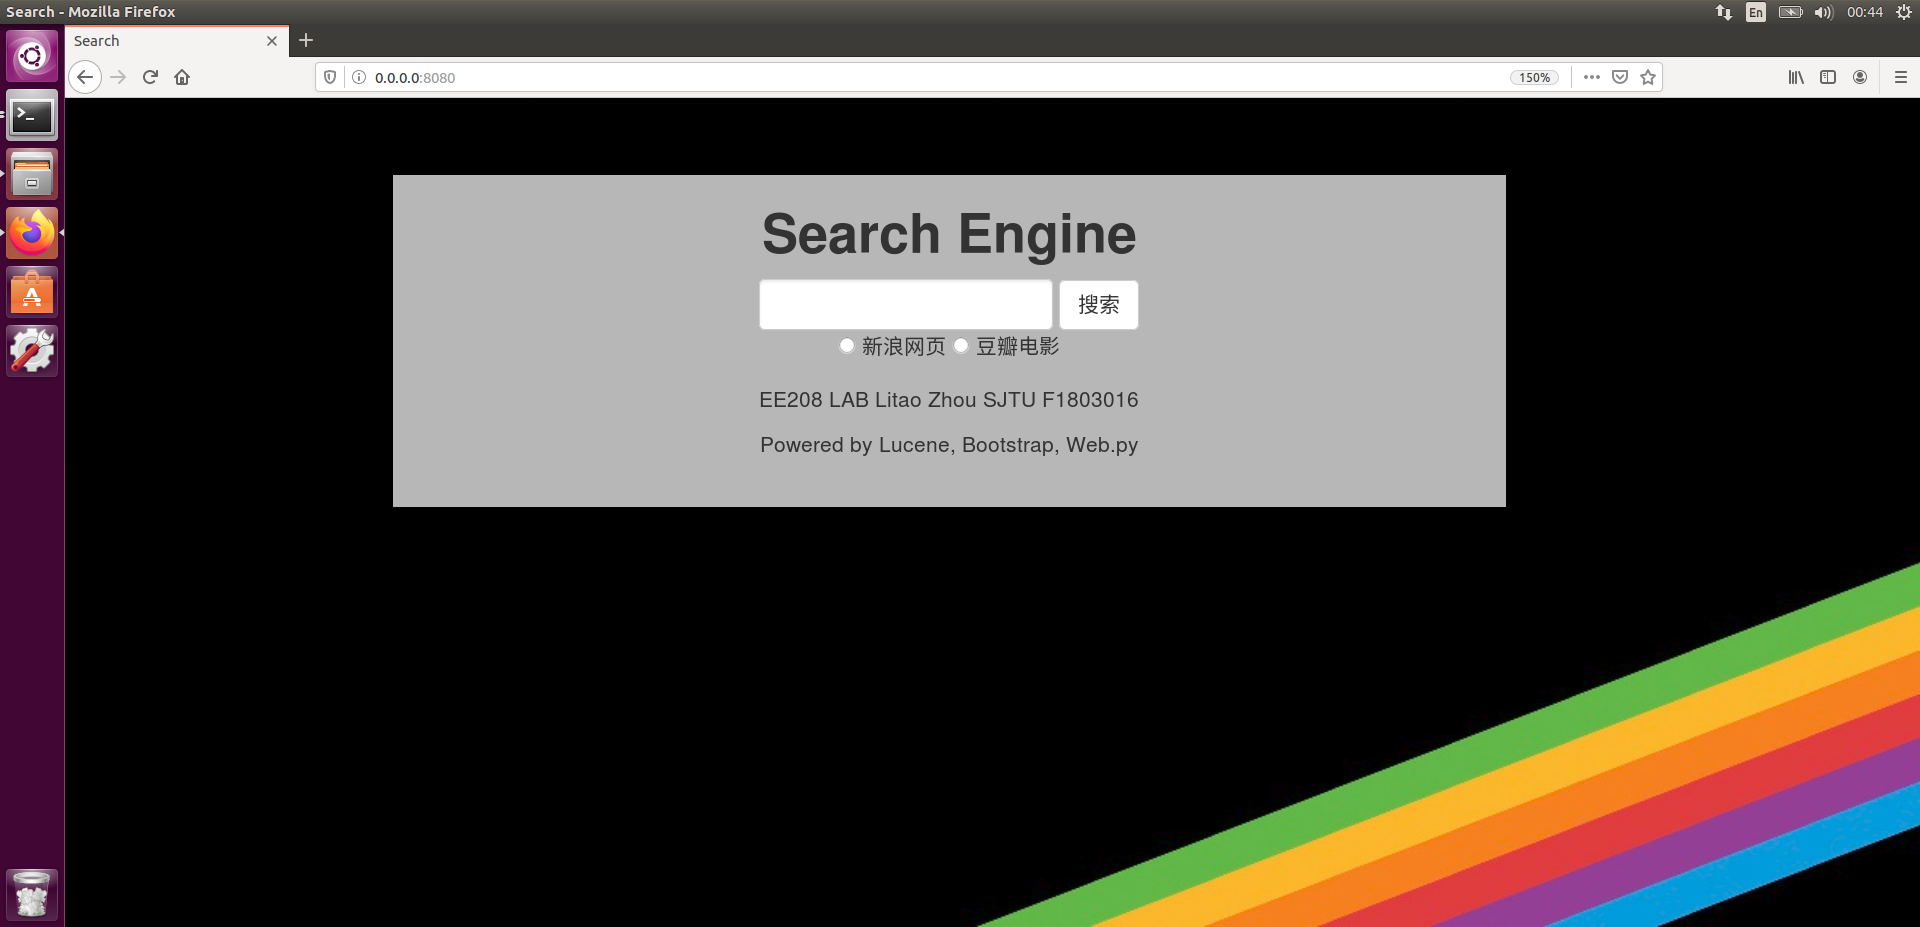
\includegraphics[width=13.5cm]{img/index.png}
\caption{主页效果展示}
\label{fig:idx}
\end{figure}


\subsection{搜索结果页的布局}

\paragraph{结果页模板} 本实验中的结果页模板既适用于网页结果,也适用于图片检索结果。页面模板包含三个参数,label(WEB/IMG)将会显示在页面中,kw(关键词)将会成为页面标题的一部分,contents是Python调用搜索程序生成的一段带HTML标签,带特定class、id标记的字符串,包含所有搜索结果需要展示的信息,将会直接成为页面的主要部分。对图片、网页两种检索操作,contents内容会带有不同的标签和类,将会进一步被外部的CSS样式表规范。结果页模板的HTML代码如下。
\begin{python}
$def with (label,kw,contents)
<html lang="zh-CN">
<head>
	# ... 调用Bootstrap样式表 ...
	<title>Search Results for $kw </title>
</head>
<body>
	<div class="container" id="result">
		<div class="row">
			<div class="col-lg-2">
				<h3>$label
				results</h3>
			</div>
			<div class="col-lg-10" style="padding-top: 15px;">
			   # form 表单
			</div>
		</div>
		<div class='result_contents'>
		  $:contents
		</div>
	</div>
	# ... 调用jQuery脚本...
</body>
</html>
\end{python}

\paragraph{结果页内容} 结果页的主要内容包含最多50条与搜索结果匹配的网页信息,包括标题、URL、带高亮的摘要。这些内容都可以从上一次实验的搜索程序中获得,running()函数将返回一个包含以上三个信息tuple的list,在Python中对这个list遍历,加上相应的标签。每一条信息都位于一个class为websec的分区中,标题带有超链接,URL和摘要分别具有weburl、webtext的class。这些class的声明将方便此后的规范操作。将所有信息通过HTML标签连接起来,我们就得到了网页内容的HTML代码。

\begin{python}
def web_func(query):
    result_seg = running(query)
    output = ''
    count = 0
    for item in result_seg:
        count += 1
        output += "<div class='websec' id='res"+str(count)+"'>"
        output += "<h3><a href='"+item[1]+"'>"+item[0]+"</a></h3>"
        output += "<p class='weburl'>"+item[1]+"</p>"
        output += "<p class='webtext'>"+item[2]+"</p>"
        output += "</div>"
    return output
\end{python}

\paragraph{摘要显示优化} 此前的实验中,输出的摘要之间存在中文分词的空格痕迹。在本实验中,我们在输出经过高亮的摘要前,先调用了Python字符串的split、join方法,去除了中文分词产生的空格,使输出的摘要清楚易读。

\paragraph{结果页格式规范}
在对结果页的CSS规范中,我们调整了标题、URL、摘要的字号、颜色、行距。值得注意的一点是,对于有些标题、URL过长的情况,我们使用了CSS中控制overflow的属性,达到了每一条记录的标题、URL都限制在一行以内的效果,多余的部分将会用省略号替代。经过以上CSS规范,结果页达到了美观的显示效果。

\begin{python}
.websec h3 
{
	color: rgb(51,122,183);
	word-break:keep-all;
	white-space:nowrap;
	overflow:hidden;         # 控制文本溢出
	text-overflow:ellipsis;
	font-size: 18px;
	margin-bottom: 4px;
}
\end{python}

结果页的显示效果如图\ref{fig:res}、\ref{fig:res2}所示。

\begin{figure}[htbp]
\centering
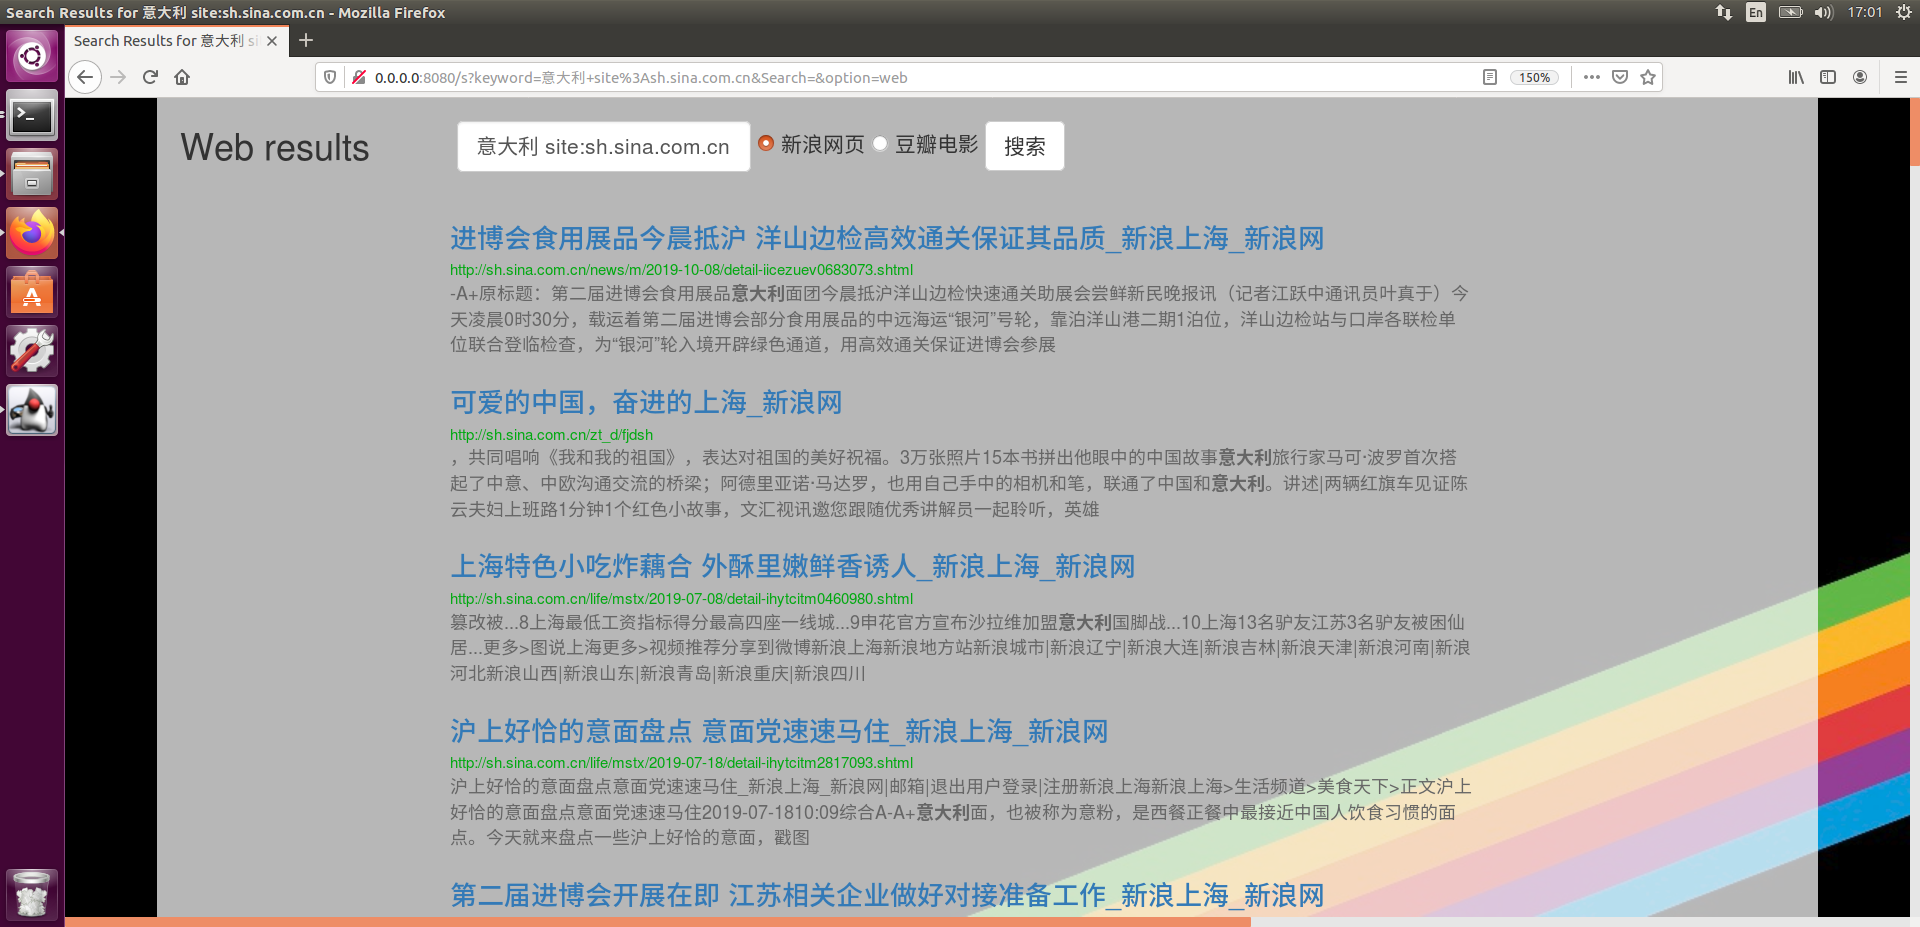
\includegraphics[width=13.5cm]{img/web.png}
\caption{网页的搜索结果页展示}
\label{fig:res}
\end{figure}

\begin{figure}[htbp]
\centering
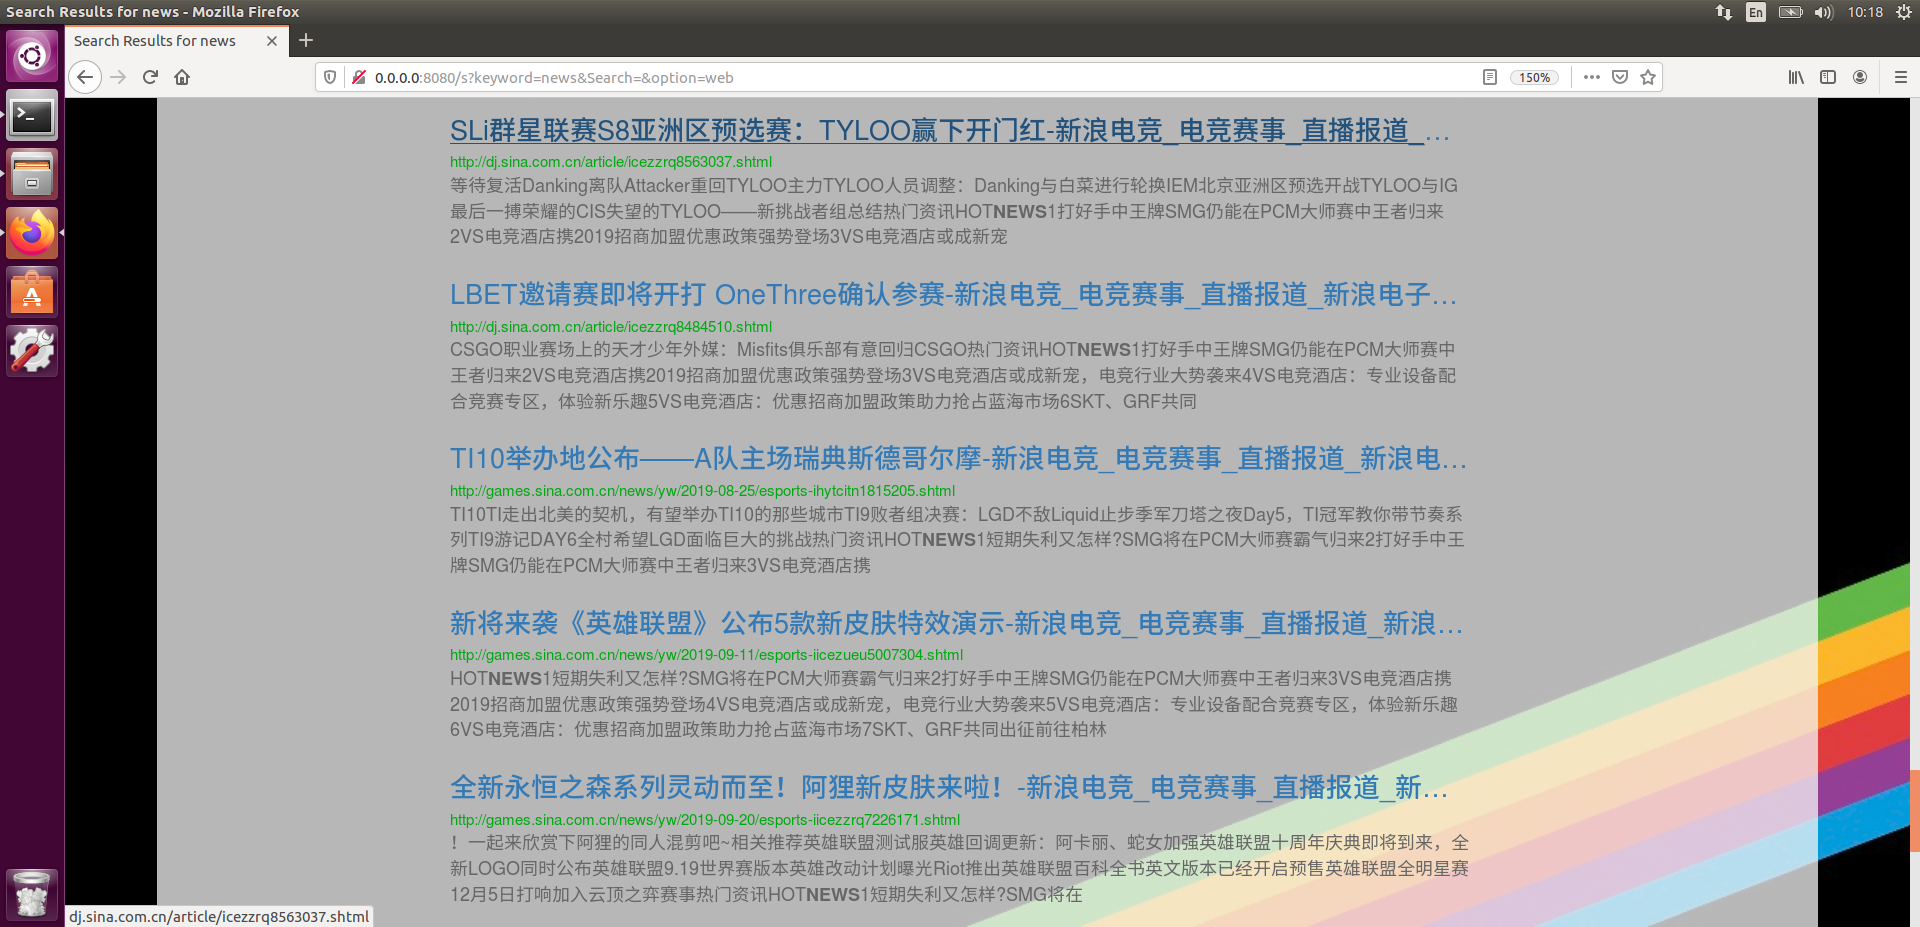
\includegraphics[width=13.5cm]{img/res2.png}
\caption{标题文本溢出时的效果}
\label{fig:res2}
\end{figure}


\subsection{图片结果页的整合}

\paragraph{图片结果页的内容} 图片结果页采用了和网页结果页一样的模板,不同之处在于传入模板的contents内容存在不同。在此前的实验中,我们已经成功搭建了图片的索引和搜索程序,搜索程序会对输入的关键词执行检索,返回图片地址、网页URL和网页标题。与前一部分实验一样,将这些信息用HTML标签连接起来,我们就可以实现图片结果页的显示。

\begin{python}
def img_func(query):
    result_seg = running(query)
    output = ''
    count = 0
    for item in result_seg:                      # item = (imgurl,url,title)
        count += 1
        output += "<div class='col-md-3'>"       # 每一个图片结果都被一个bootstrap分区包围
        output += "<div class='imgsec' id='res"+str(count)+"'>"
        output += "<a class='thumbnail' href='"+item[1]+"'>"          
                         # 图片本身的超链接标签指向页面URL,用bootstrap中thumbnail类进行规范。
        output += "<img class='img-responsive' src='"+item[0]+"' alt='"+item[2]+"'> </img>"
        output += "<p class='imgtext'>"+item[2]+"</p></a>"        
        output += "</div></div>"
    return output
\end{python}

\paragraph{图片结果页的规范} 排版图片页面的主要困难在于图片尺寸大小不一,无法合理有序地排布在页面中,为此我们在外部CSS样式表中规定了图片的高度尺寸。使所有图片框的大小都能保持一致。对于图片的依次排列,我们采用了Bootstrap中的列分块(col-md-3),Bootstrap的排版系统中,将网页各区域横向分为12个列,此处我们对每张图片使用3列宽的空间,就能实现4张图片一行的依次排布。当页宽较小时,如在手机浏览器中,Bootstrap还能自动调整为紧凑的排布方式。最终图片页的排版效果如图\ref{fig:img}所示。

\begin{figure}[htbp]
\centering
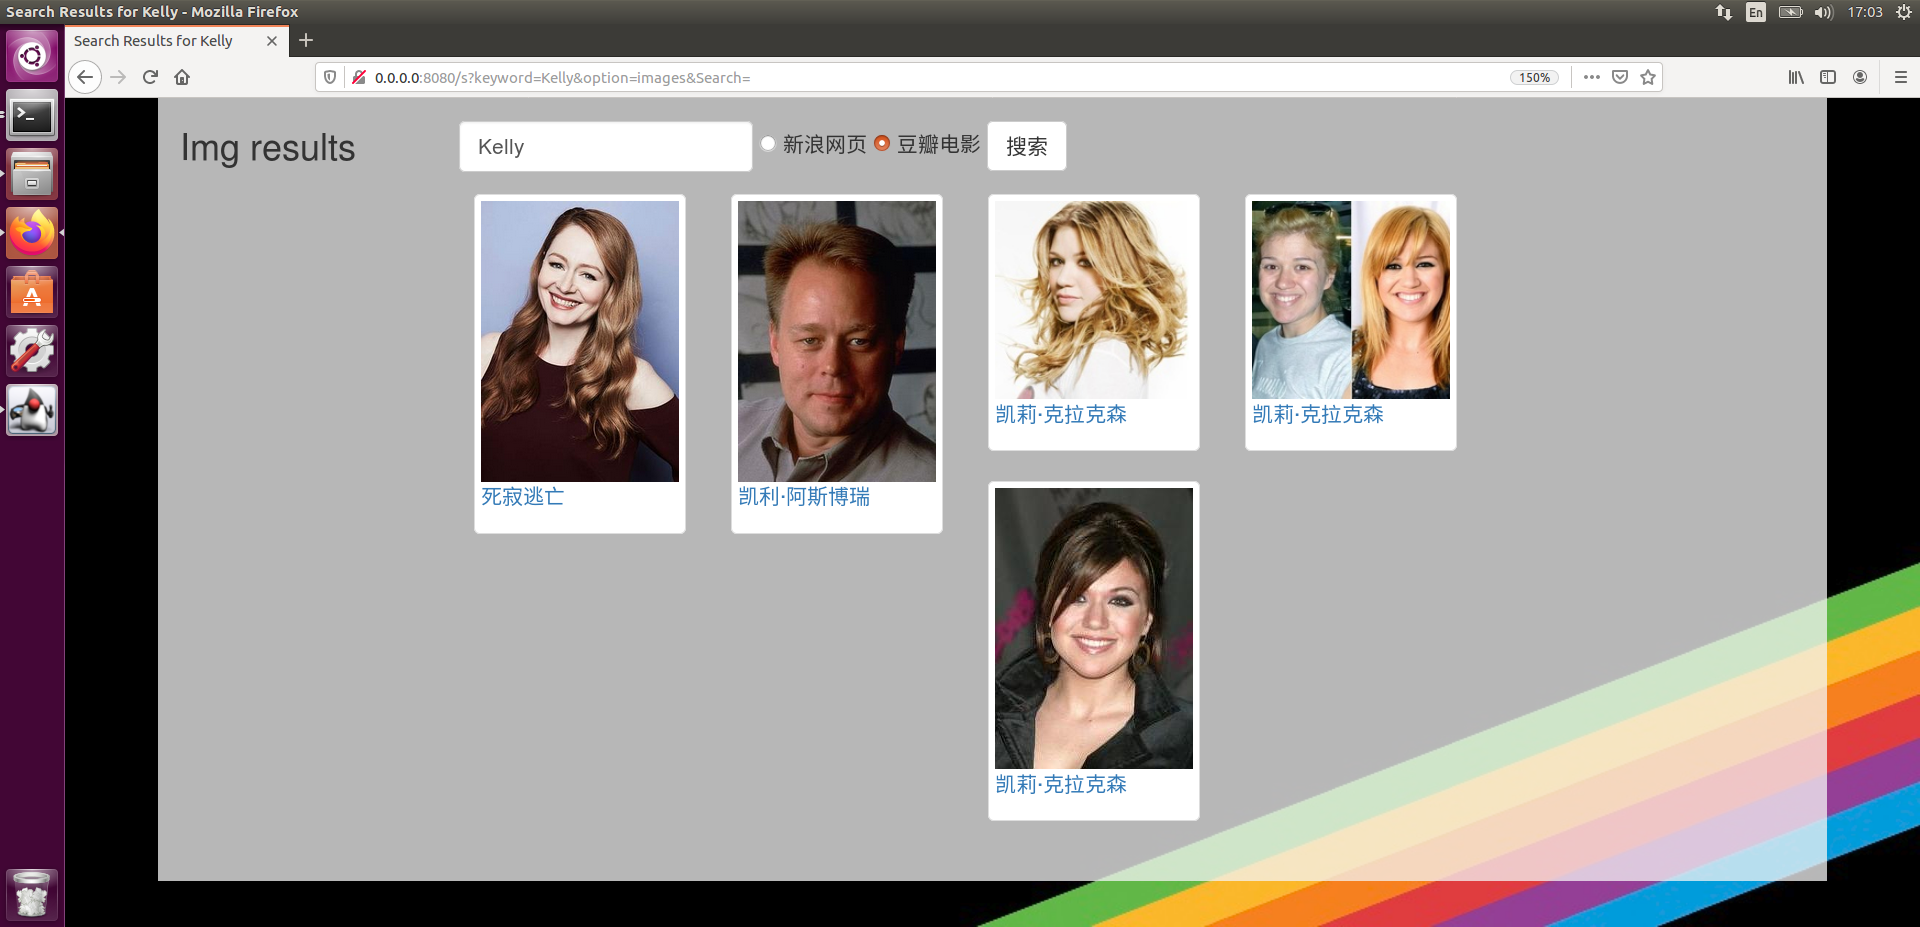
\includegraphics[width=13.5cm]{img/img2.png}
\caption{网页的搜索结果页展示}
\label{fig:img}
\end{figure}



\section{实验总结}
\paragraph{概述}
本实验中,我们将此前的爬虫、网页解析、建立索引、搜索程序、web前端等知识整合到一起,搭建了一个较为完整的网页+图片搜索引擎,同时利用div+CSS对格式进行了美化和规范。

\paragraph{感想}
通过本次实验的学习,我回顾了此前搜索引擎搭建的知识,对过去的代码进行了进一步的整合、优化,完善了我对搜索引擎搭建流程的认识。此外,我也在实践的过程中,学习了不少CSS排版的技巧和思路。

\paragraph{创新}
在本实验中,我在用网页前端整合此前实验成果的同时,也对Highlightsearch、PictSearch脚本做了整合和优化。在前端网页规范方面,我通过引入Bootstrap的样式表,使排版更加美观高效,达到了更好的整合效果。

\paragraph{问题}

在实验的进行过程中,我遇到的第一个问题是在模板中调用外部运行目录下style.css样式表时,web.py会提示找不到文件报错,这是因为web.py在生成网页时,会将网页存放于运行目录下的/static文件夹中,因此通过将外部样式表、背景图片移动到新建的static文件夹中,就可以解决上述问题。另外,在图片搜索结果页中,会遇到豆瓣电影图片无法显示的情况,我们需要对网页头文件中的referer稍加设置,可以解决这一问题。
\begin{python}
<meta name="referrer" content="never">
\end{python}

除了以上问题外,本实验还有可以进一步有待优化的地方,比如对网页内容的输出,本实验中采取了在Python中用字符串操作将各条信息连接起来统一输出HTML代码的方式,一个更好的实现是直接将包含信息的list输出,在模板中使用web.py的for语句对结果进行遍历,这将使输出形式更为灵活,移植性更好。这是在未来实验或者大作业中可以改善的方向。


\end{document}

